\documentclass[10pt,a4paper]{article}
\usepackage[margin=14mm,top=10mm,bottom=15mm]{geometry}
\usepackage[T1]{fontenc}
\usepackage{lmodern}
\usepackage{microtype}
\usepackage{booktabs}
\usepackage{array}
\usepackage{xcolor}
\usepackage[hidelinks]{hyperref}
\usepackage{tabularx}
\usepackage{tikz}
\usepackage{graphicx}
\usetikzlibrary{arrows.meta}

\usepackage{graphicx}
\renewcommand{\normalsize}{\fontsize{9.4}{11.3}\selectfont}
\renewcommand{\small}{\fontsize{8.6}{10.3}\selectfont}
\normalsize
\setlength{\parskip}{2.5pt}
\makeatletter\renewcommand\section{\@startsection{section}{1}{\z@}{3pt}{1.5pt}{\normalfont\large\bfseries}}\makeatother
\let\olditemize\itemize\renewcommand{\itemize}{\olditemize\setlength{\itemsep}{1pt}\setlength{\parsep}{0pt}\setlength{\topsep}{2pt}\setlength{\leftmargin}{1.2em}}
\setlength{\parindent}{0pt}
\renewcommand{\arraystretch}{1.08}
\definecolor{accent}{RGB}{46,107,75}
\definecolor{amber}{RGB}{154,106,31}
\definecolor{brick}{RGB}{165,67,44}
\definecolor{soft}{RGB}{231,240,233}
\newcommand{\gate}[1]{\textcolor{accent}{\textbf{#1}}}
\newcommand{\todo}[1]{\textcolor{red}{[#1]}}
\newcommand{\ok}{\textcolor{accent}{clean}}
\newcommand{\okm}{\textcolor{accent}{match}}
\newcommand{\dens}{\textcolor{accent}{density only}}
\newcommand{\nr}{\textcolor{amber}{to run}}
\newcommand{\mm}{\textcolor{brick}{mismatch}}

\begin{document}

{\LARGE\bfseries USYD SoC Design Challenge -- Agriculture SoC}\\[1pt]
{\large Timeline and verification plan to tapeout 7 December 2026}\\[2pt]
{\small Prepared by Lewis Watts for the team, 21 September 2026 \;$\cdot$\; \href{https://github.com/lewisMW/agriculture-SoC}{github.com/lewisMW/agriculture-SoC}}

\vspace{3pt}\hrule\vspace{3pt}

\section*{Summary}
We are taping out a mixed-signal precision-agriculture SoC using an Arm Cortex-M0 subsystem on the SoCLabs NanoSoC platform with an 8-bit, 100\,kS/s SAR ADC front end on the ChipFoundry chipIgnite \texttt{ci2612} shuttle (SkyWater SKY130). The project began in ELEC3607 (2024 S1) and competes in the SoCLabs SoC Design Contest (Educational Implementation track).

\textbf{Project Status:} the full digital chip is synthesised, placed, routed and timing-closed at 33\,MHz; the ADC is verified at transistor level from firmware running on the Cortex-M0 (Fig.~1); every analog cell has a schematic and layout, DRC is essentially clean and LVS is under way.
\textbf{Funding:} S3B provides AU\$21{,}000 against a US\$14{,}500 shuttle. \textbf{Key dates:} 50\,\% commit \textbf{8 October} (flexible), tapeout \textbf{7 December} (fixed).

\section{Status and Recent Achievements}
\begin{minipage}[t]{0.56\textwidth}
\vspace{0pt}
\begin{itemize}
\item \textbf{Digital implementation (Daniel Geng).} Cadence Genus synthesis and Innovus place-and-route of the SoC: Cortex-M0, four 8\,kB SRAMs, SKY130 pad ring (Fig.~2).
\\
\textbf{Timing closed post-route at 33\,MHz} and closing DRC violations.
\item \textbf{Mixed-signal co-verification (Ben Schwarz \& Lewis Watts).} C firmware on the Cortex-M0 triggers SAR ADC conversions over the ARM core's APB bus. The analog components use SKY130 transistor-level cells solved by Cadence Spectre running within an Xcelium AMS simulation. Six self-checking firmware tests (validated on a deliberately broken design) produce ADC codes within 1 to 2\,LSB of the behavioural model.
\item \textbf{Analog cells in SKY130 (Hee Chan Kim Cabrera, Erick Gomez Landeros Acosta, Jaime Pryor).} All eight analog modules have AKY130-specific schematics and layouts and are DRC-clean, apart from density rules that will be resolved by chip fill in the integration stage. LVS has started, 50\% progress.
\item \textbf{Independent reviewers:} Kushal Das (Senior Cryogenic ASIC Engineer, USyd Nano Institute): analog, already mentoring the SAR design; Daniel Newbrook (Senior ASIC/FPGA Design Engineer, University of Southampton / SoCLabs): SKY130 flow and Cortex-M0 integration; Samuel Tensingh: SKY130 Cadence flow.
\end{itemize}
\end{minipage}\hfill
\begin{minipage}[t]{0.41\textwidth}
\vspace{0pt}
\centering
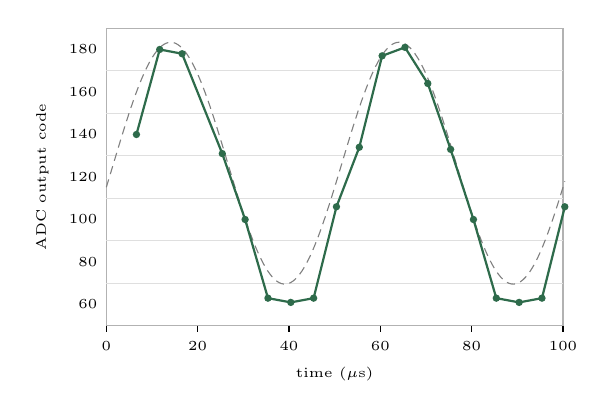
\begin{tikzpicture}[x=0.058cm,y=0.027cm]
  % axes: x = time (us) 0..100 ; y = code 50..190
  \draw[gray!60] (0,50) rectangle (100,190);
  \foreach \y in {70,90,...,170} \draw[gray!25] (0,\y) -- (100,\y);
  \foreach \y in {60,80,...,180} \node[left,font=\tiny] at (0,\y) {\y};
  \foreach \x in {0,20,...,100} { \draw (\x,50) -- (\x,47); \node[below,font=\tiny] at (\x,47) {\x}; }
  \node[below,font=\tiny] at (50,35) {time ($\mu$s)};
  \node[rotate=90,font=\tiny] at (-14,120) {ADC output code};
  % ideal 8-bit response to the +/-0.8 V differential input; sampling instant and offset fitted to the 5 kHz run (<1 LSB)
  \draw[gray,densely dashed] plot[domain=0:100.4,samples=200,smooth] (\x,{126.5+56.9*sin(7.2*(\x-1.6))});
  % act 3 (adc_trigger_test, SENSING_DEBUG fifo_push trace), FIN_HZ=20e3 by -defparam, 25 Sep
  \draw[accent,thick] plot[mark=*,mark size=0.9pt] coordinates {
    (6.6,140)(11.7,180)(16.6,178)(25.4,131)(30.4,100)(35.4,63)(40.4,61)(45.4,63)(50.4,106)(55.4,134)(60.4,177)(65.4,181)(70.4,164)(75.4,133)(80.4,100)(85.4,63)(90.4,61)(95.4,63)(100.4,106)};
\end{tikzpicture}\\[-2pt]
{\footnotesize\textbf{Fig.~1.} Codes read by the Cortex-M0 from the transistor-level SAR ADC (Spectre in the loop) for a 20\,kHz differential sine (dashed: ideal). The sine's troughs bias towards 0x3F, which is consistent with a known switch-recharge effect at twice the rated conversion rate, to be fixed.}

\vspace{8pt}
{\small\textbf{Budget} (AU\$, US\$ at 1.4035 mid on 21 Sep)}\\[-2pt]
{\small
\begin{tabularx}{\textwidth}{@{}X r@{}}
\toprule
chipIgnite ci2612 slot, incl.\ eval PCB (US\$14{,}500) & 20{,}350 \\
\quad 50\,\% commit, 8 Oct (US\$7{,}250) & 10{,}175 \\
\quad balance at tapeout, 7 Dec (US\$7{,}250) & 10{,}175 \\
FX transfer fees (est.\ 3.0\,\%) & 610 \\
Connectors, consumables (balance) & 200 \\
\midrule
Total cost & 21{,}000 \\
S3B funding & $-$21{,}000 \\
\midrule
\textbf{Balance (AU\$)} & \textbf{160} \\
\bottomrule
\end{tabularx}}
\end{minipage}

\section{Timeline: Milestones to Tapeout}
\begin{center}
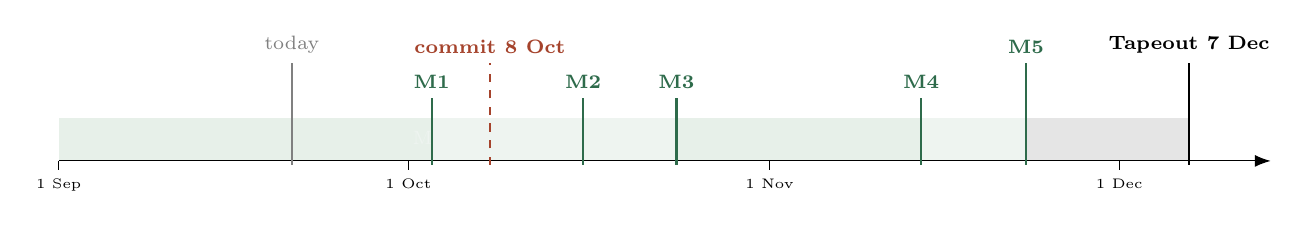
\begin{tikzpicture}[x=0.148cm,y=1cm]
  % day 0 = 1 Sep 2026; 7 Dec = day 97
  \fill[soft] (0,0) rectangle (32,0.55) node[midway,font=\scriptsize] {M1 consolidate};
  \fill[soft!70] (32,0) rectangle (53,0.55) node[midway,font=\scriptsize] {M2 ADC macro + extraction};
  \fill[soft] (53,0) rectangle (74,0.55) node[midway,font=\scriptsize] {M3 chip integration};
  \fill[soft!70] (74,0) rectangle (83,0.55) node[midway,font=\scriptsize] {M4 sign-off};
  \fill[gray!20] (83,0) rectangle (97,0.55) node[midway,font=\scriptsize] {buffer};
  \draw[-{Latex[length=2mm]}] (0,0) -- (104,0);
  \foreach \d/\l in {0/1 Sep,30/1 Oct,61/1 Nov,91/1 Dec} { \draw (\d,0) -- (\d,-0.12); \node[below,font=\tiny] at (\d,-0.12) {\l}; }
  \foreach \d/\l/\h in {32/M1/0.8,45/M2/0.8,53/M3/0.8,74/M4/0.8,83/M5/1.25} { \draw[accent,thick] (\d,-0.05) -- (\d,\h); \node[above,font=\scriptsize\bfseries,accent] at (\d,\h) {\l}; }
  \draw[brick,thick,dashed] (37,-0.05) -- (37,1.25); \node[above,font=\scriptsize\bfseries,brick] at (37,1.25) {commit 8 Oct};
  \draw[black,thick] (97,-0.05) -- (97,1.25); \node[above,font=\scriptsize\bfseries] at (97,1.25) {Tapeout 7 Dec};
  \draw[gray,thick] (20,-0.05) -- (20,1.25); \node[above,font=\scriptsize,gray] at (20,1.25) {today};
\end{tikzpicture}
\end{center}
\vspace{-6pt}
\begin{tabularx}{\textwidth}{@{}l X@{}}
\gate{M1} 3 Oct & LVS passes on all analog modules; ADC macro layout + parasitic extraction, the simulation of which still passes the 6 self-checking firmware tests in mixed-signal co-verification. \\
\gate{M2} 10 Oct & The MVP of the ADC macro is provided for integration into the synthesis flow. \\
\gate{M3} 24 Oct & Achieve ADC figure of merits including: INL/DNL $<$ 1\,LSB, no missing codes, ENOB $\ge$ 7 at 100\,kS/s across process/temperature/supply corners, and a process-based Monte-Carlo simulation produces voltage offsets within the configurable trim range. \\
\gate{M4} 14 Nov & Full-chip DRC/LVS/antenna clean; firmware regression tests passes with the full extracted ADC in the loop. Gate level simulation passes. \\
\gate{M5} 23 Nov & Sign-off checklist reviewed with Kushal Das, Daniel Newbrook and Samuel Tensingh with two weeks of buffer. GDS submitted 7 Dec. \\
\end{tabularx}

\begin{center}
\resizebox{0.93\textwidth}{!}{%
\begin{tikzpicture}[x=1cm,y=1cm]
  % ---- chip render: image covers -34.42..3476.71 um (x) and -34.42..4076.33 um (y) at 6.0 cm width
  \pgfmathsetmacro{\s}{5.4/3511.13}
  \node[anchor=south west,inner sep=0] at (0,0) {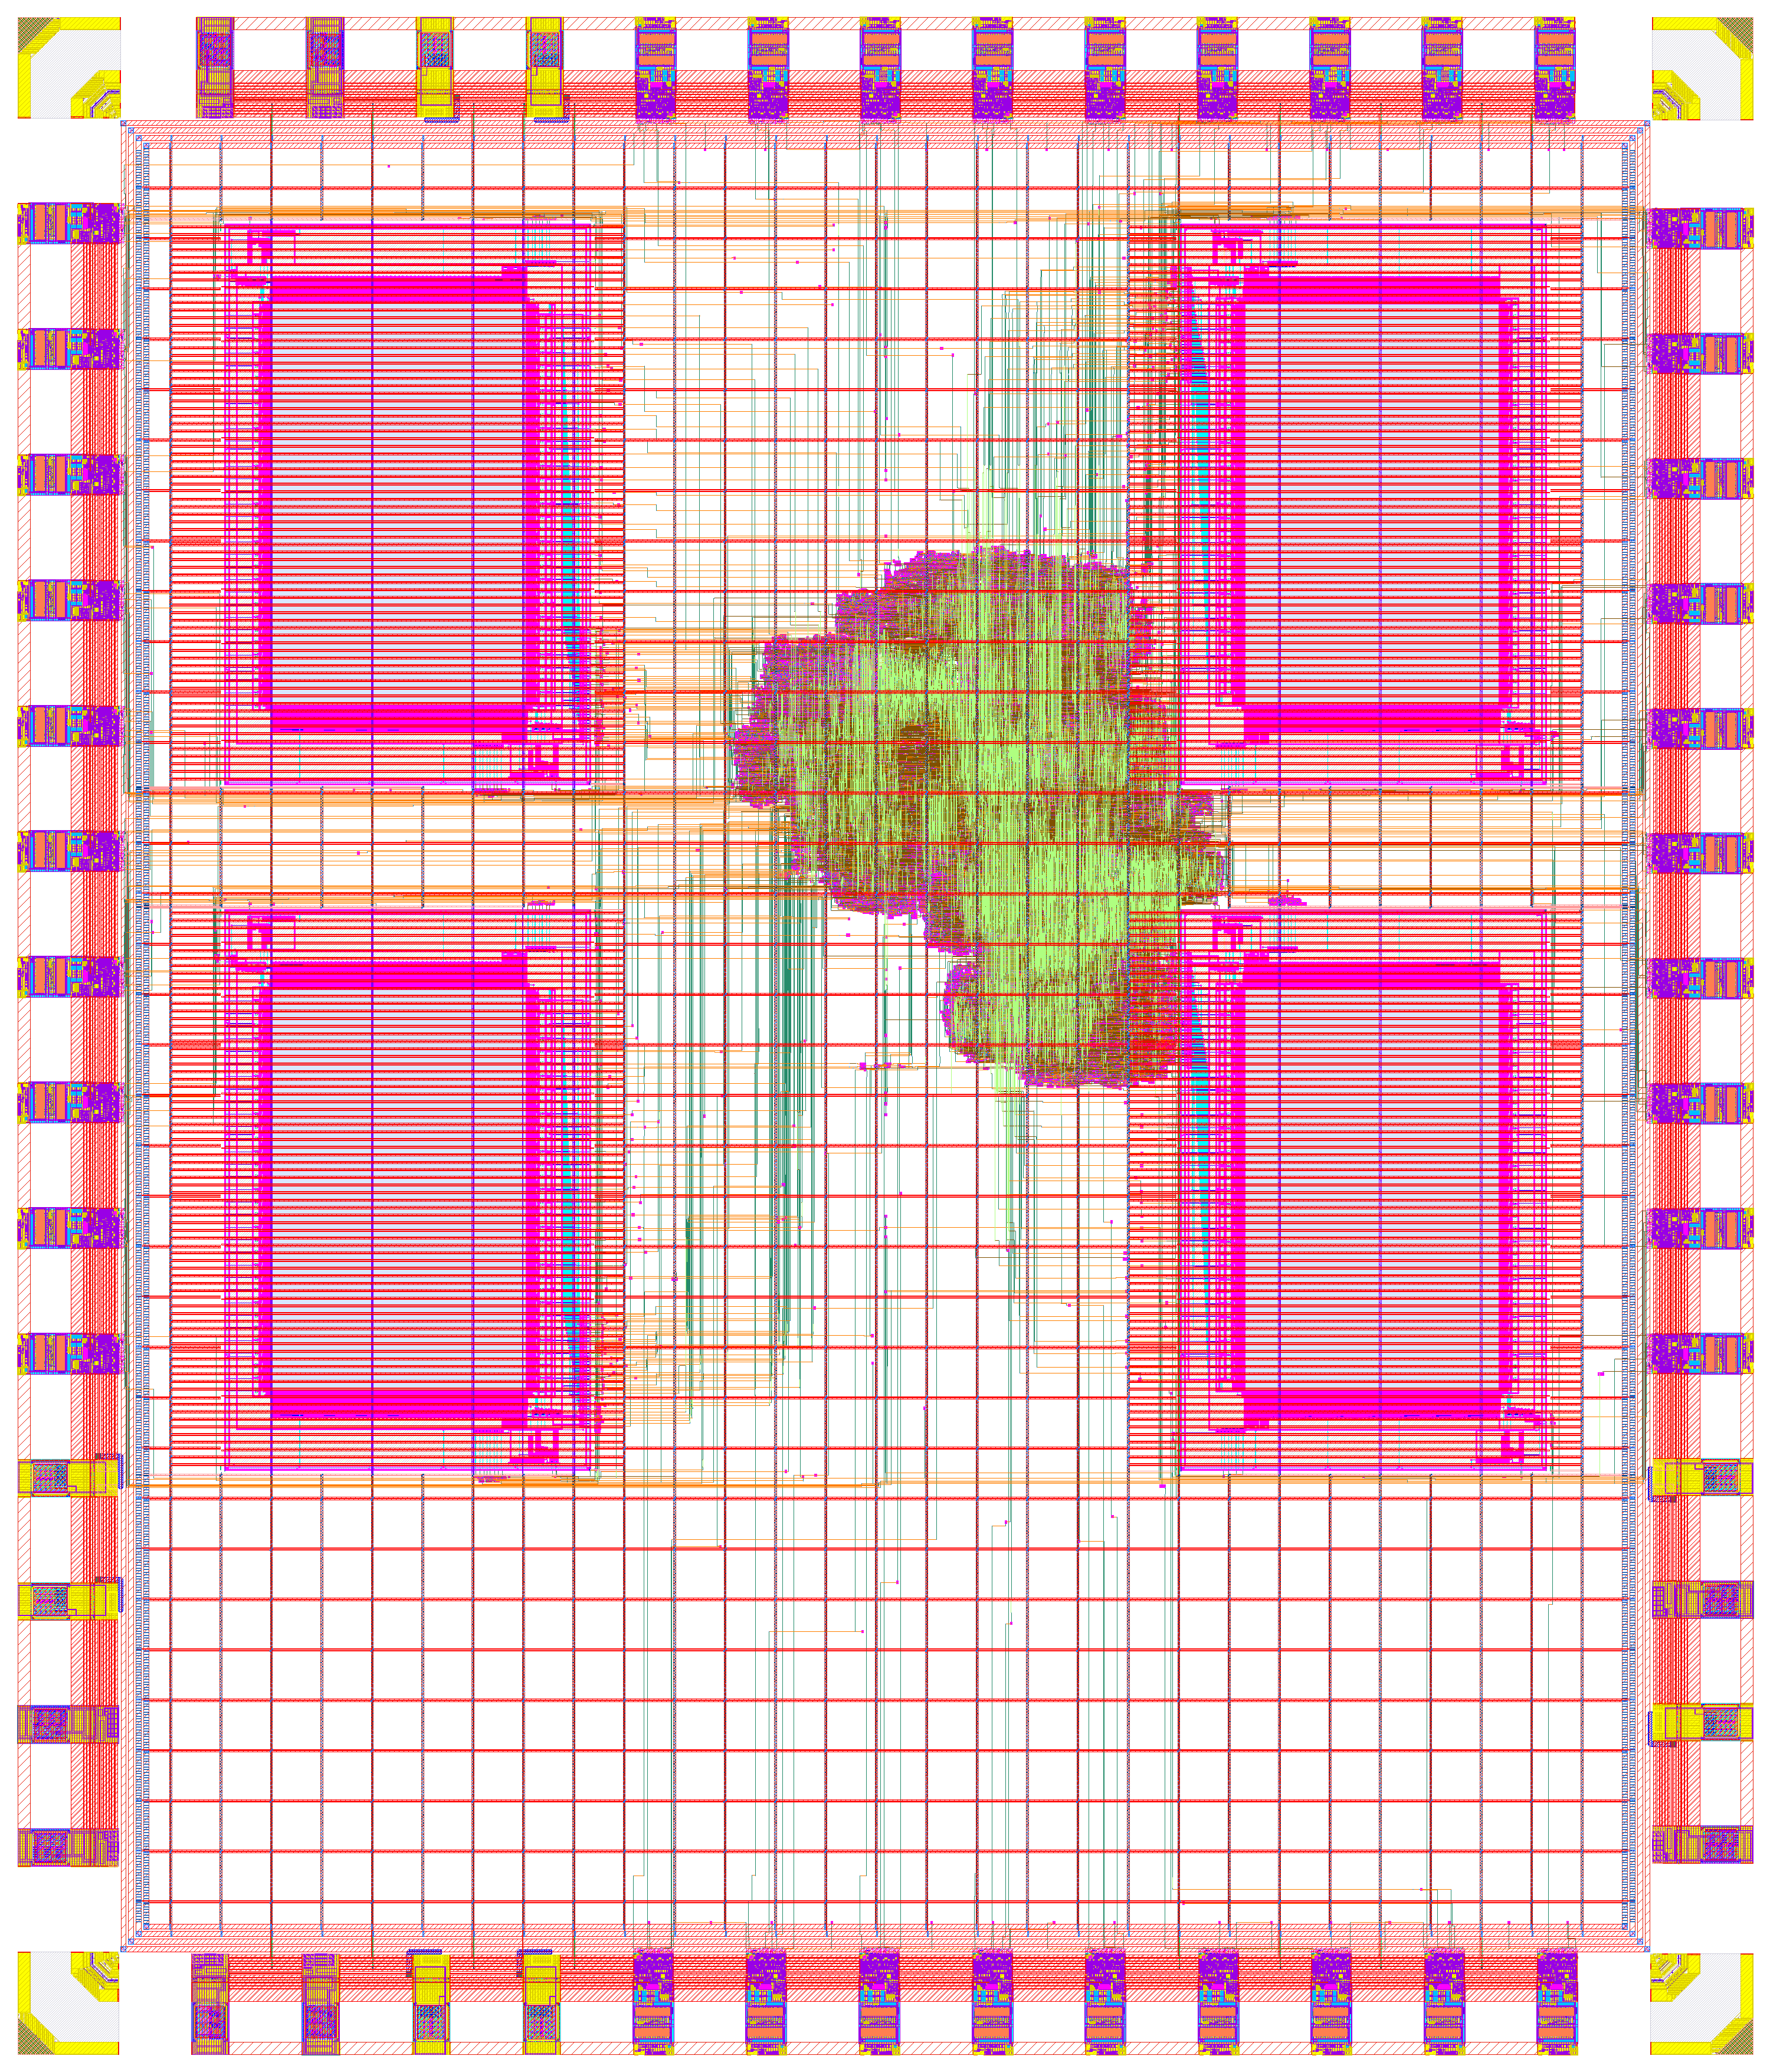
\includegraphics[width=5.4cm]{fig/chip_routed.png}};
  \begin{scope}[shift={(34.42*\s,34.42*\s)},x=\s cm,y=\s cm]
    % callout boxes (um), Daniel's 22 Sep GDS: SRAM instance bboxes; Cortex-M0 = extent of u_cortexm0 placements,
    % which reach into the channel between the right-hand SRAMs
    \draw[accent,thick] (2307,1160) rectangle (3031,2270);
    \draw[accent,thick] (2307,2520) rectangle (3031,3631);
    \draw[accent,thick] (411,1160) rectangle (1135,2270);
    \draw[accent,thick] (411,2520) rectangle (1135,3631);
    \draw[brick,thick] (1787,1917) -- (2307,1917) -- (2307,2270) -- (2391,2270) -- (2391,2520) -- (2307,2520) -- (2307,2690) -- (1787,2690) -- cycle;
    % % ADC reserved region with the real cells at true scale
    % \draw[accent,very thick,dashed] (480,420) rectangle (980,920);
    % \pgfmathsetmacro{\wcdac}{140.6*\s}\pgfmathsetmacro{\wcmp}{43.4*\s}\pgfmathsetmacro{\wbsw}{27.5*\s}\pgfmathsetmacro{\wtrim}{14.4*\s}
    % \node[anchor=south west,inner sep=0] at (520,470) {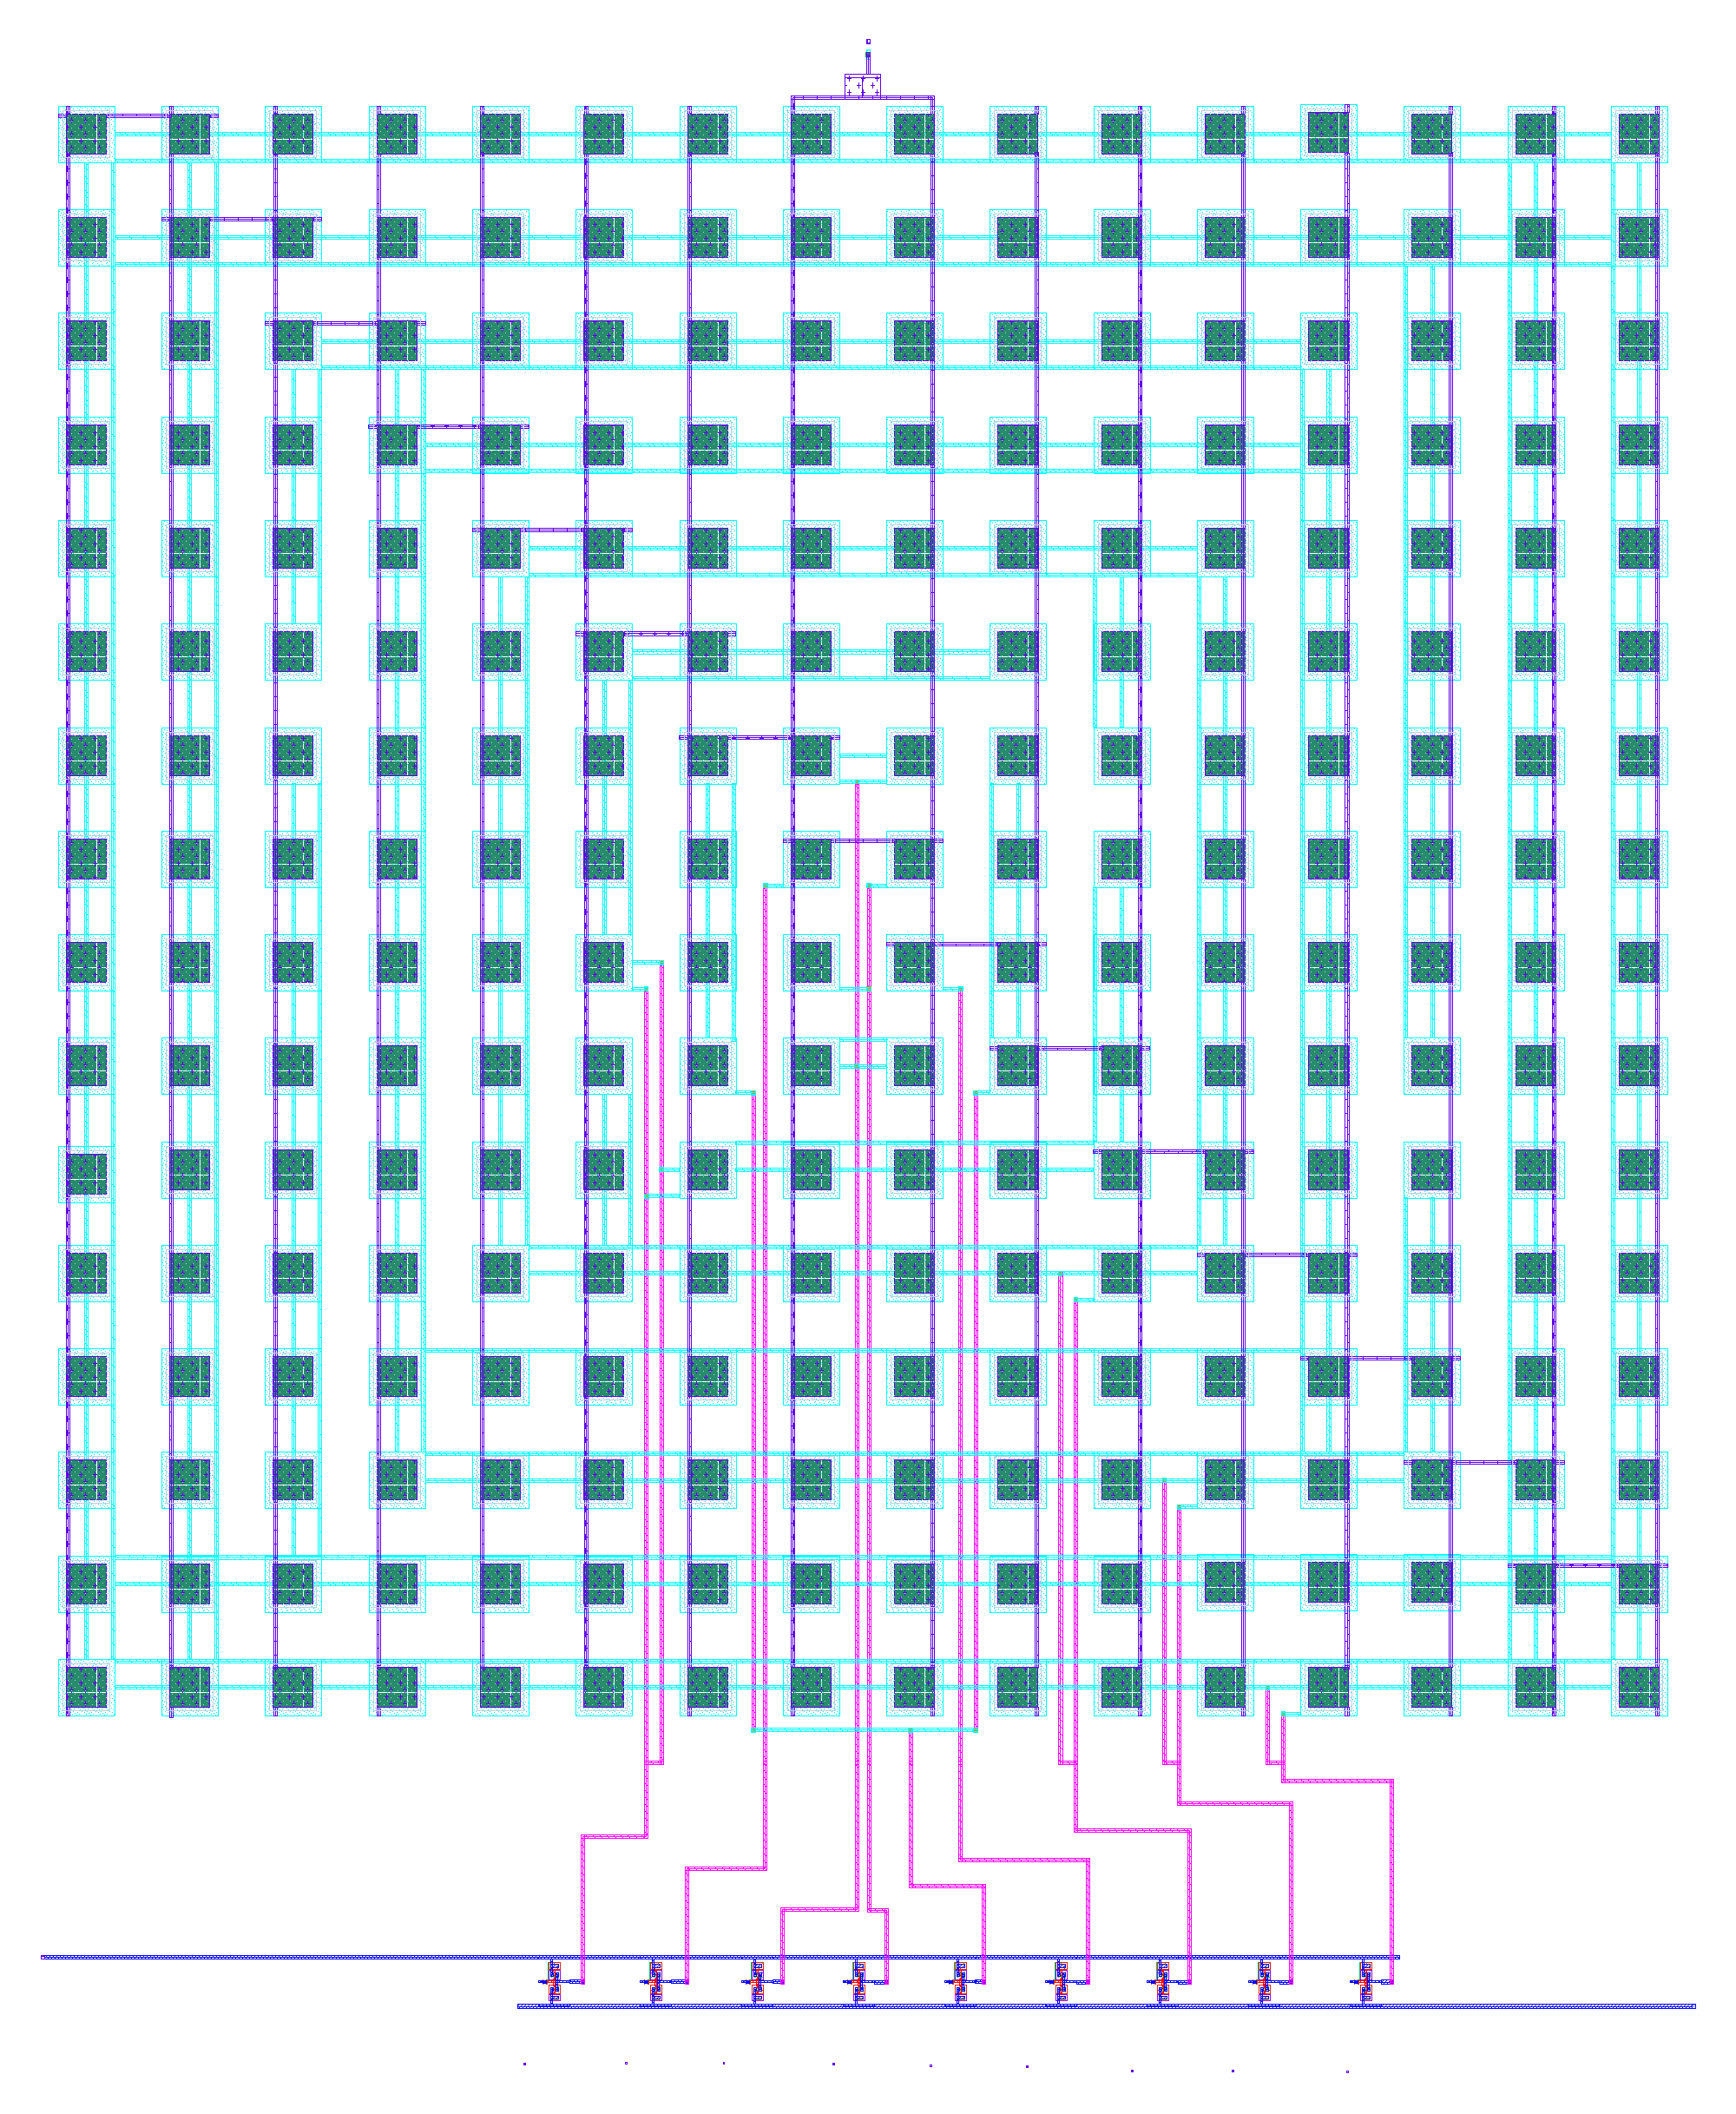
\includegraphics[width=\wcdac cm]{fig/cdac_8b.png}};
    % \node[anchor=south west,inner sep=0] at (720,470) {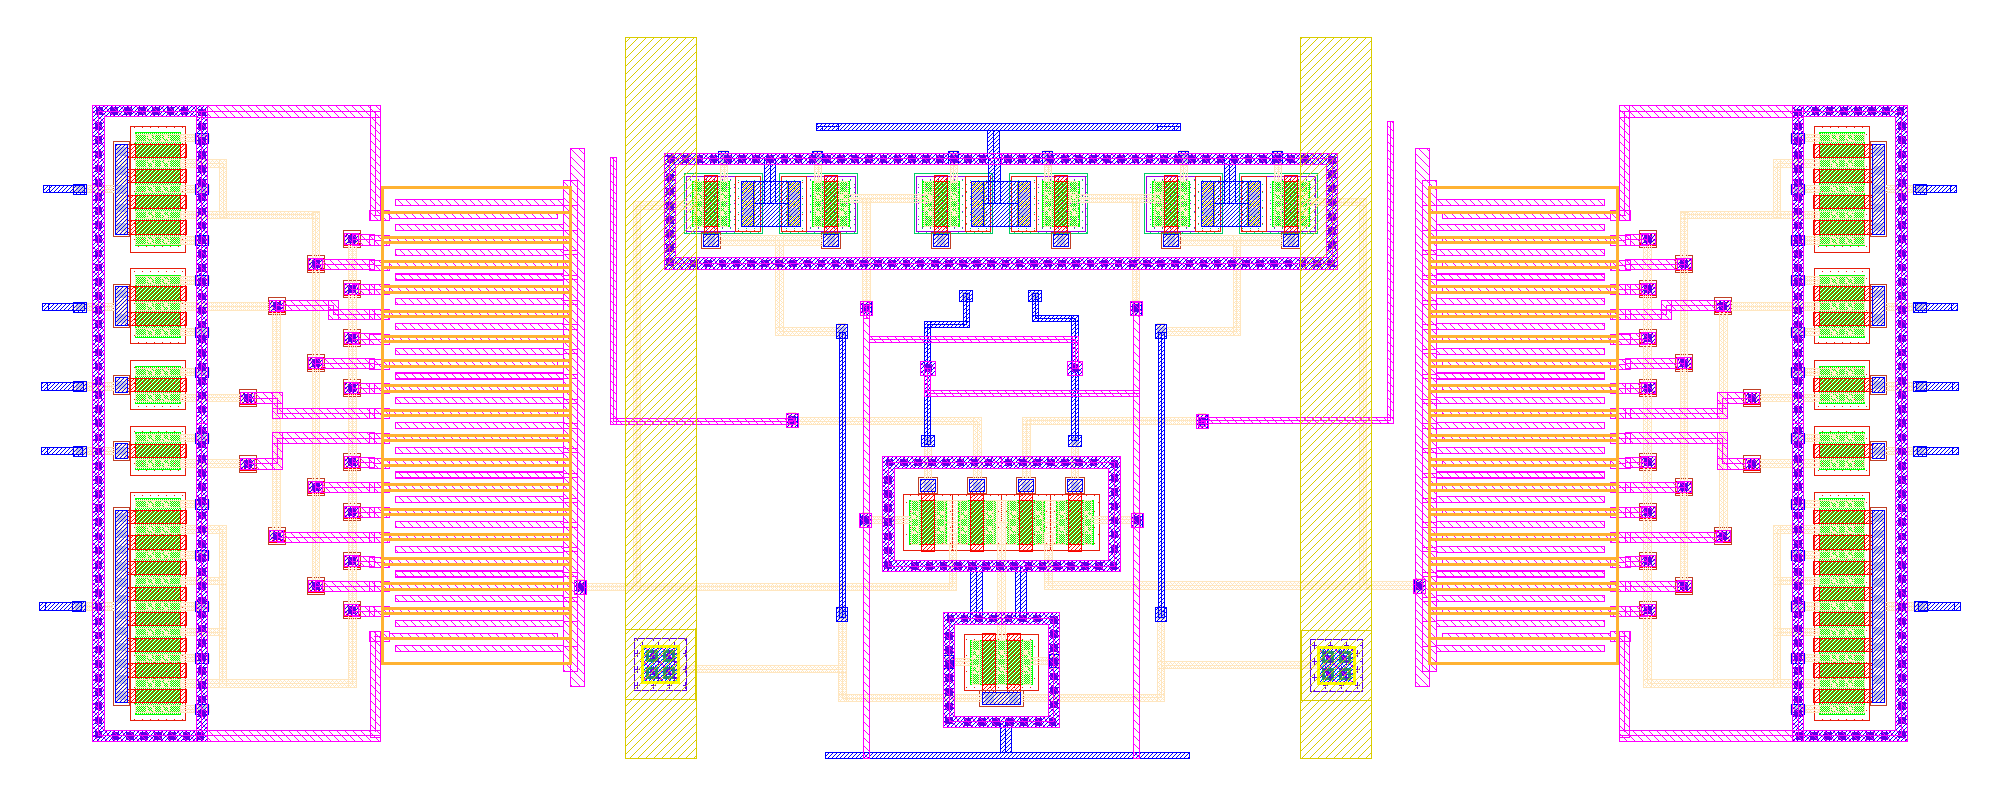
\includegraphics[width=\wcmp cm]{fig/comparator.png}};
    % \node[anchor=south west,inner sep=0] at (720,520) {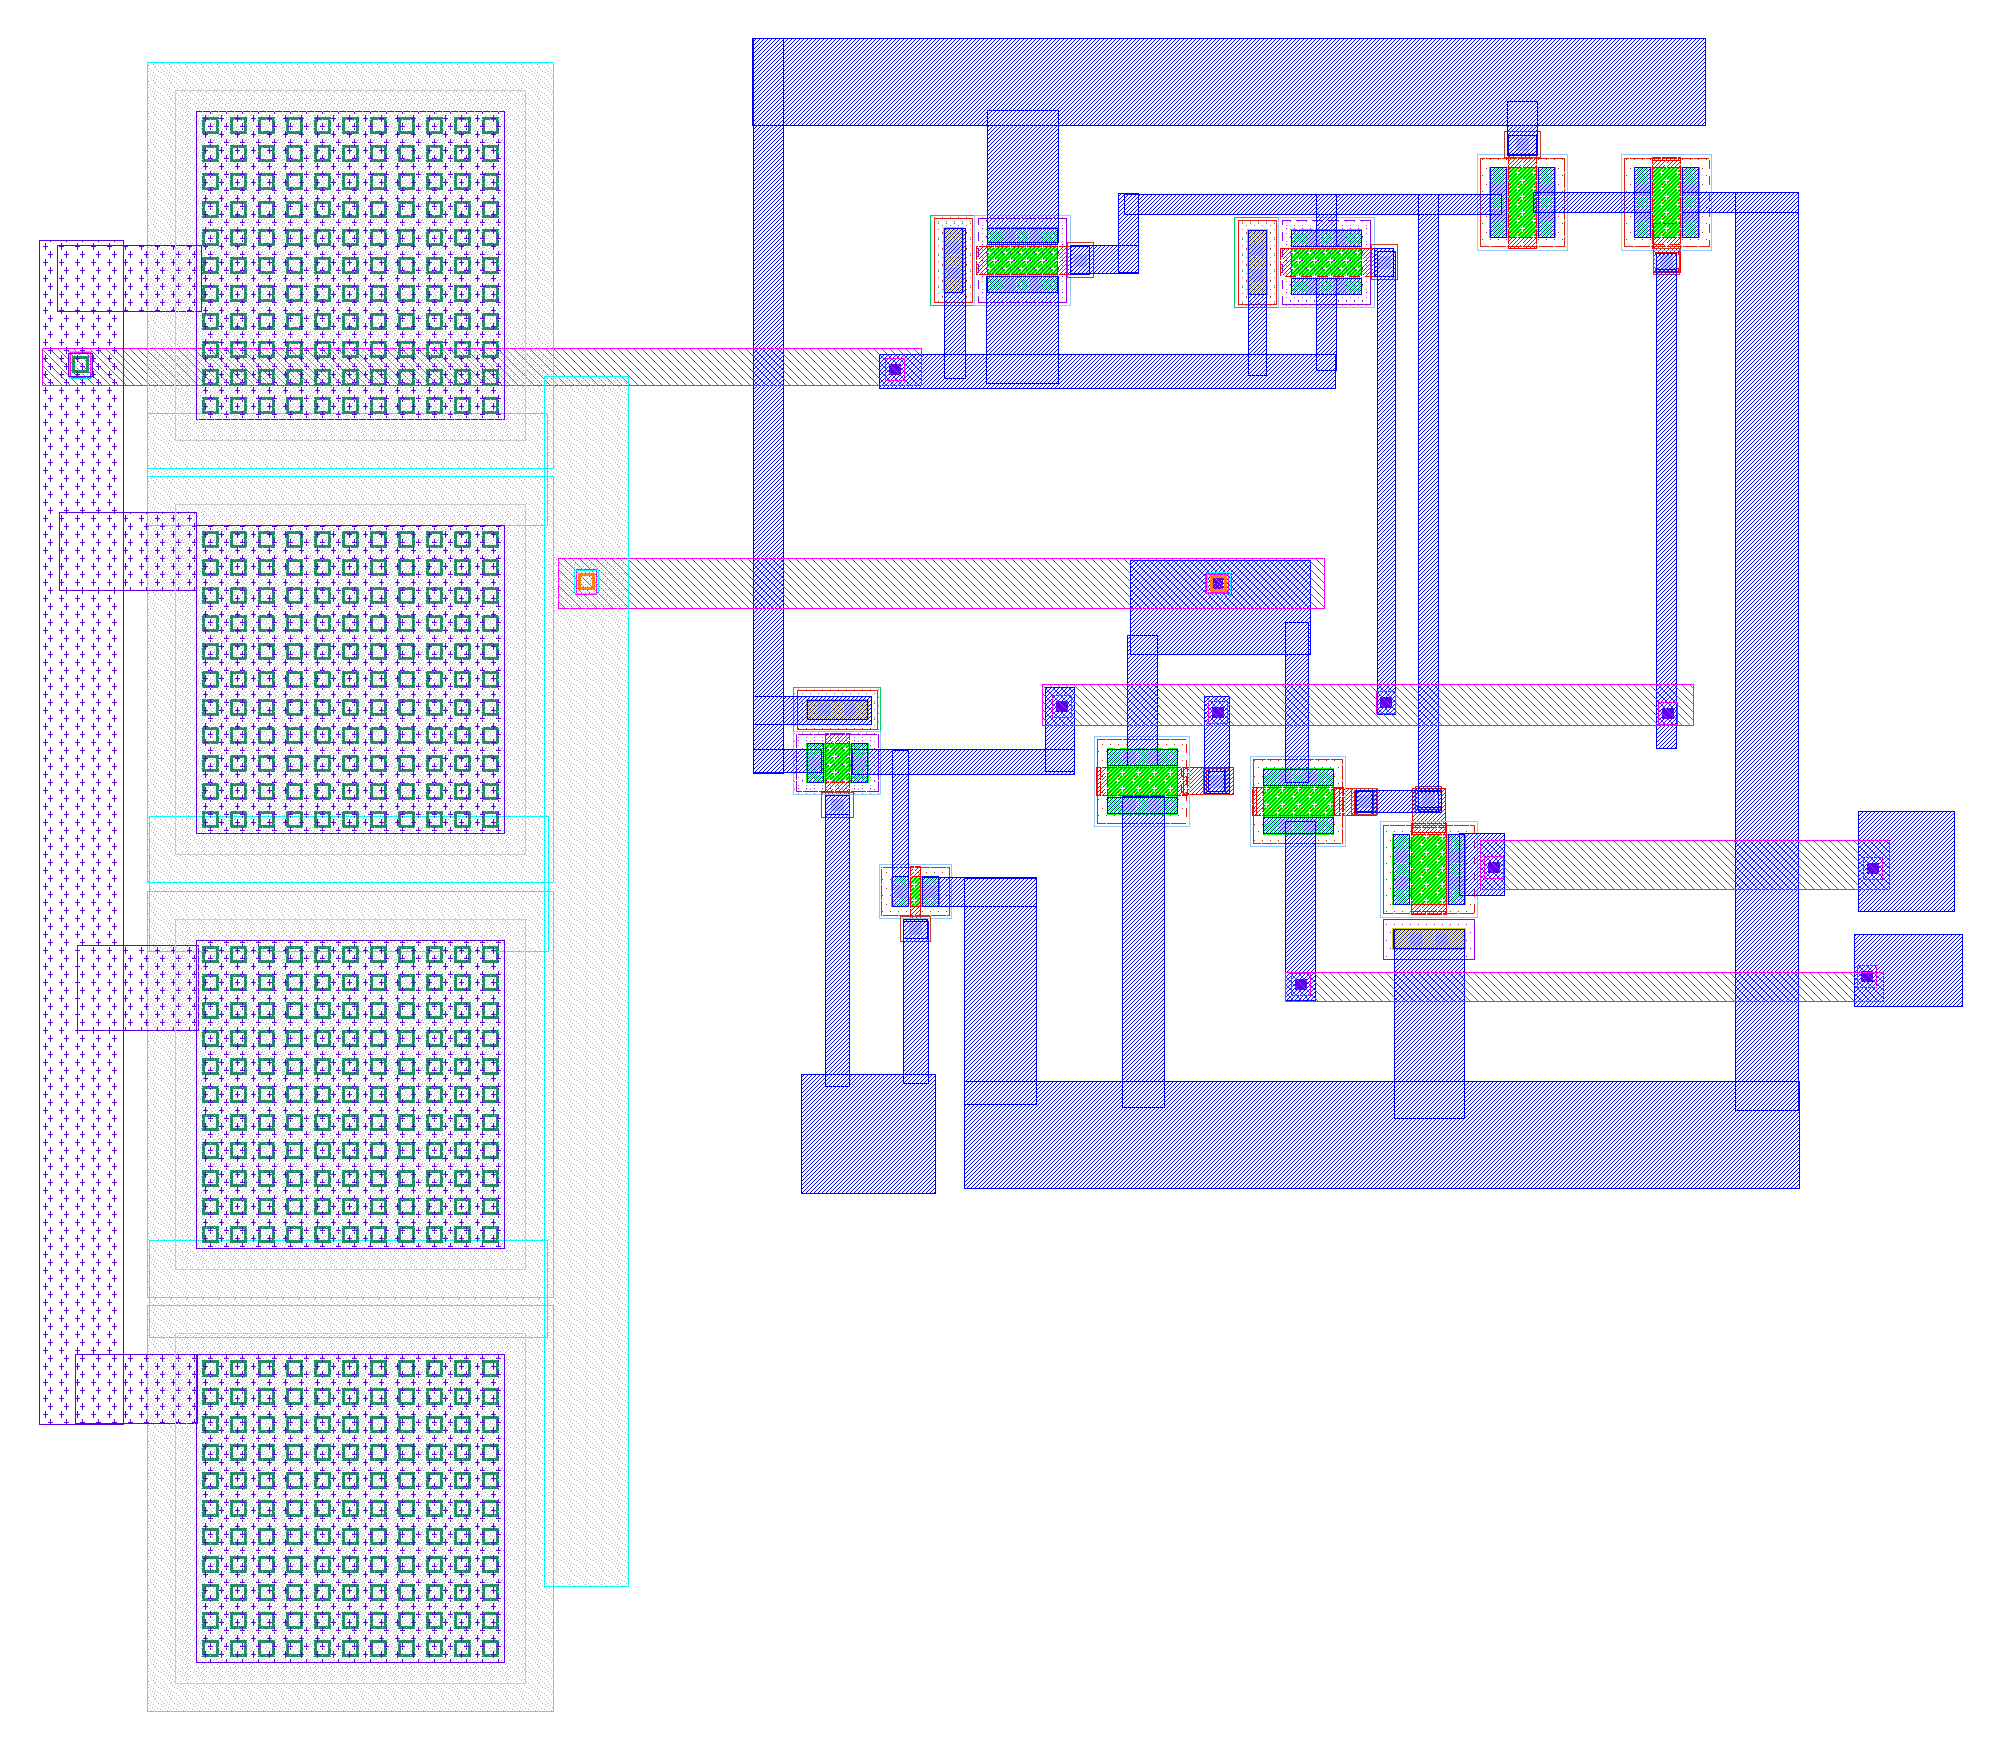
\includegraphics[width=\wbsw cm]{fig/bootstrap_sw.png}};
    % \node[anchor=south west,inner sep=0] at (780,520) {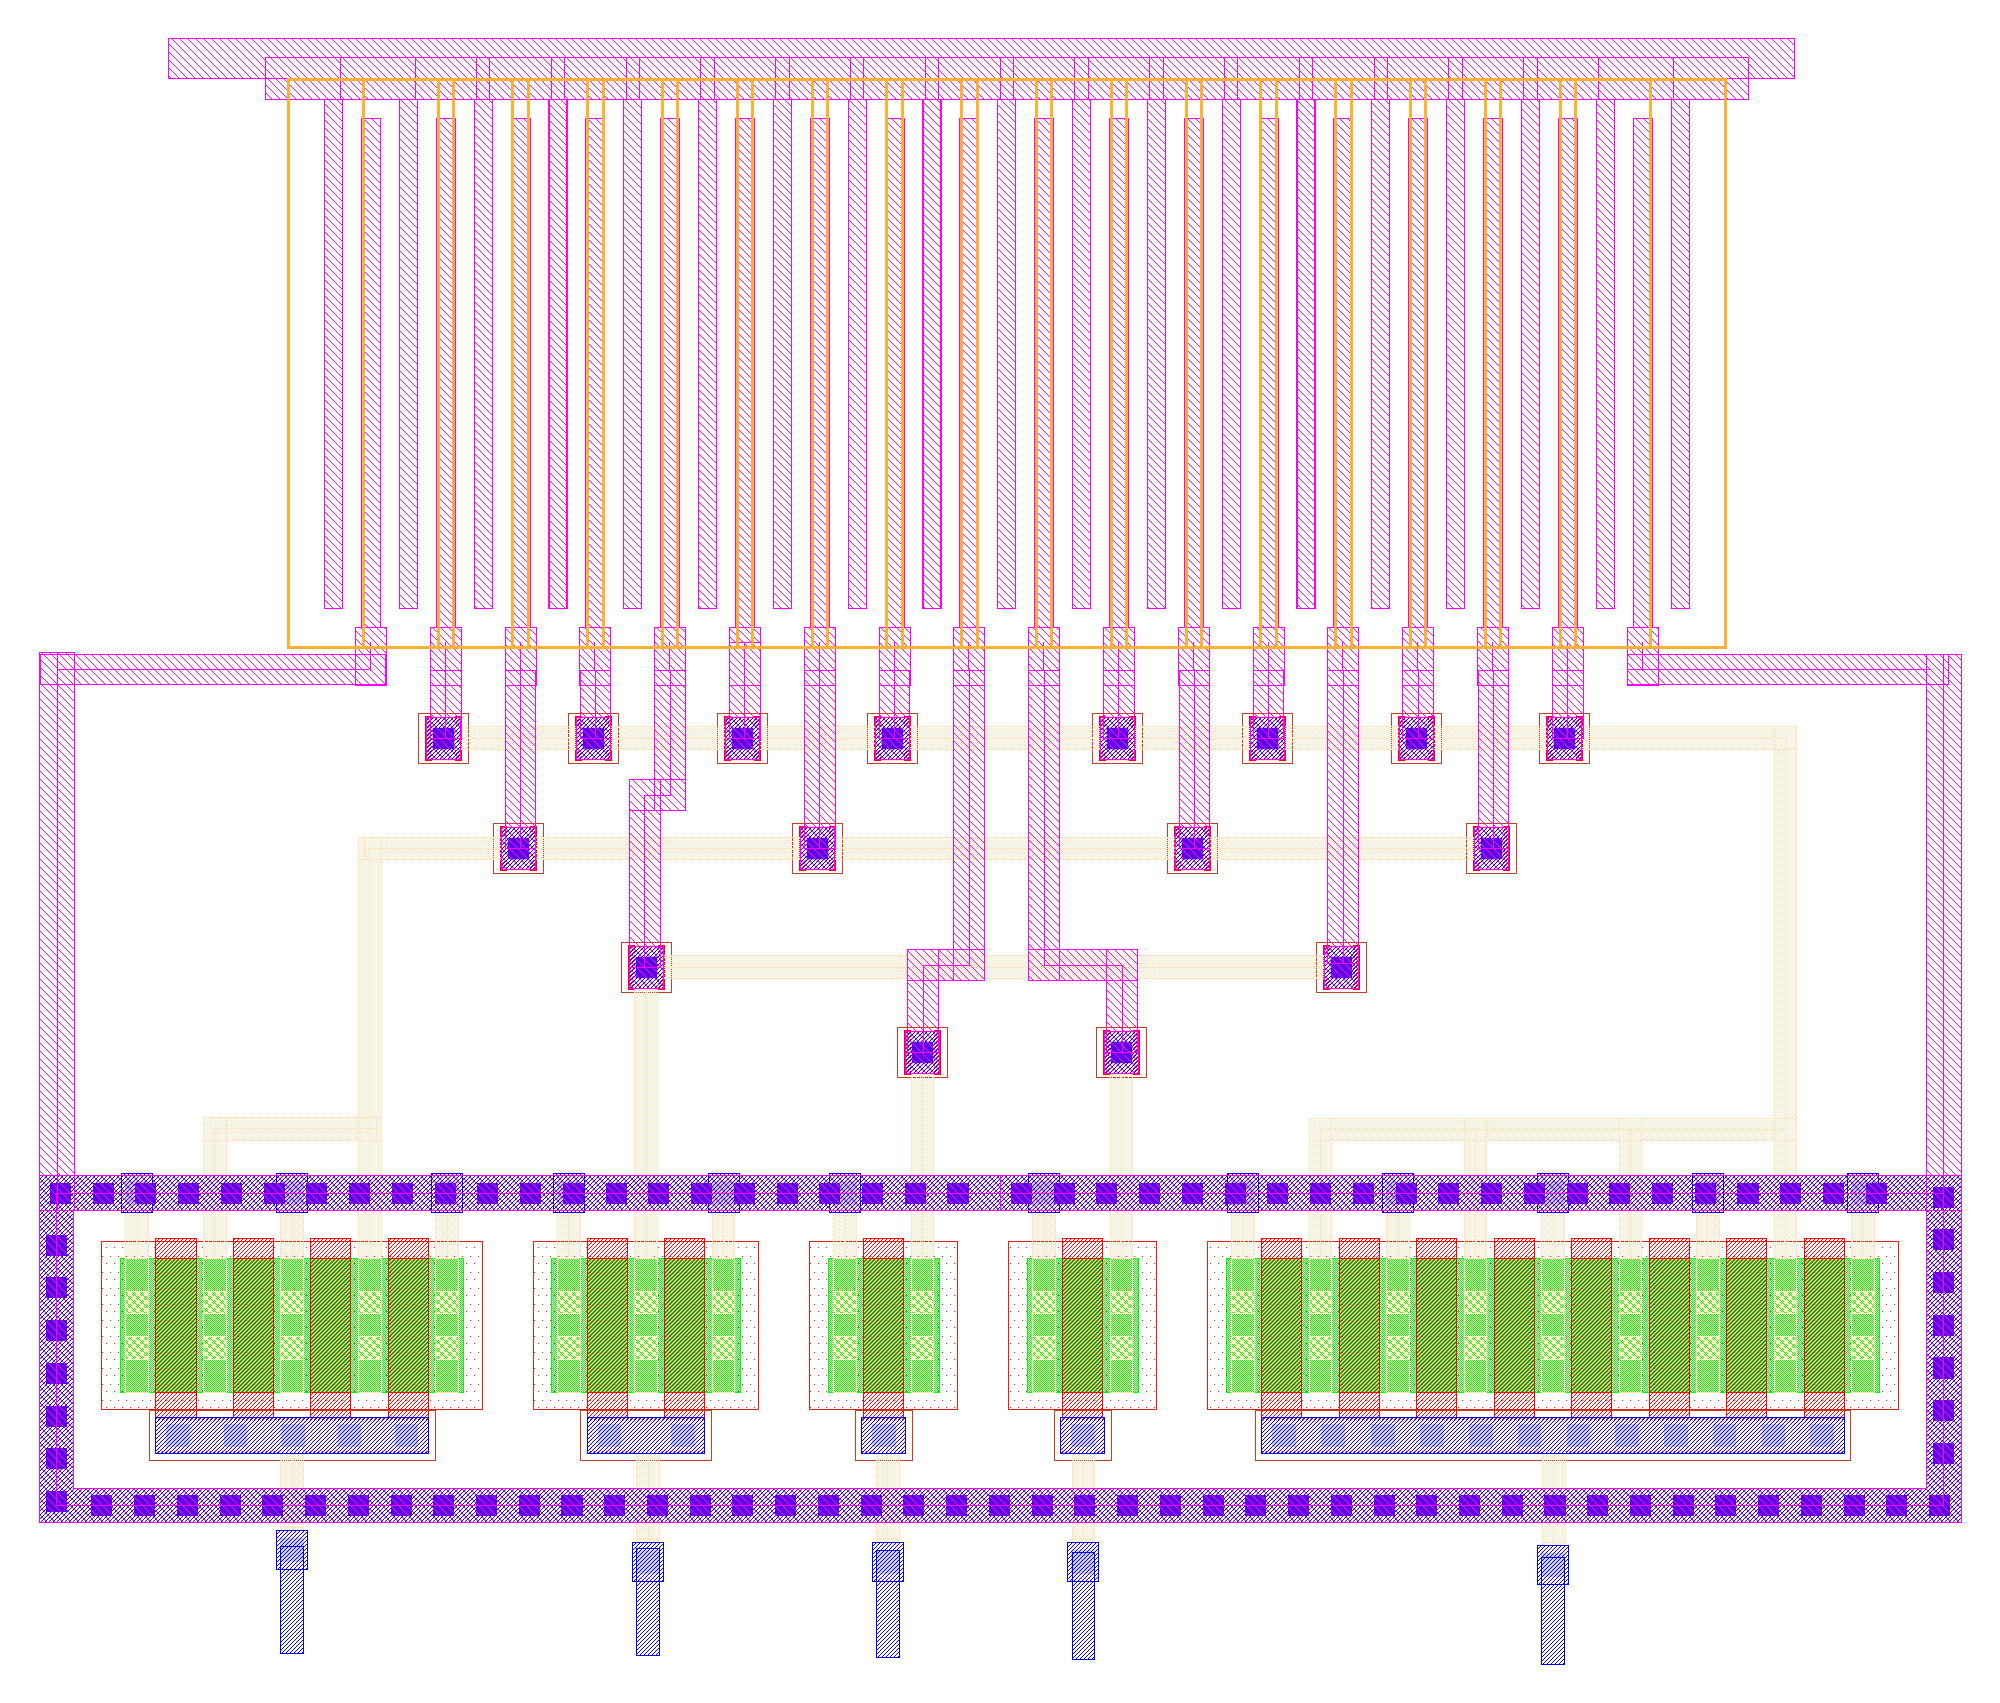
\includegraphics[width=\wtrim cm]{fig/trim.png}};
    % scale bar
    \draw[very thick] (2000,350) -- (2000+1000,350); \node[above,font=\tiny] at (2500,350) {1\,mm};
  \end{scope}
  % labels (cm coordinates; chip spans x 0..5.4, y 0..6.32)
  \node[font=\scriptsize\bfseries,accent,anchor=west] at (5.65,5.75) {4 $\times$ 8\,kB SRAM};
  \draw[accent] (5.65,5.75) -- (4.6,5.45);
  \node[font=\scriptsize\bfseries,anchor=west] at (5.65,4.45) {bus fabric, peripherals};
  \draw (5.65,4.45) -- (3.3,4.45);
  \node[font=\scriptsize\bfseries,brick,anchor=west] at (5.65,3.74) {Cortex-M0};
  \draw[brick] (5.65,3.74) -- (3.73,3.74);
  % \node[font=\scriptsize\bfseries,accent,anchor=west] at (5.65,0.85) {ADC macro (G2), true scale};
  % \draw[accent] (5.65,0.85) -- (1.58,1.08);
  \node[font=\scriptsize\bfseries,anchor=south] at (2.7,6.34) {sky130 I/O pad ring};
  % ---- right panel: the four analog cells rendered from their sky130 GDS
  \node[anchor=south west,inner sep=0] at (9.9,3.6) {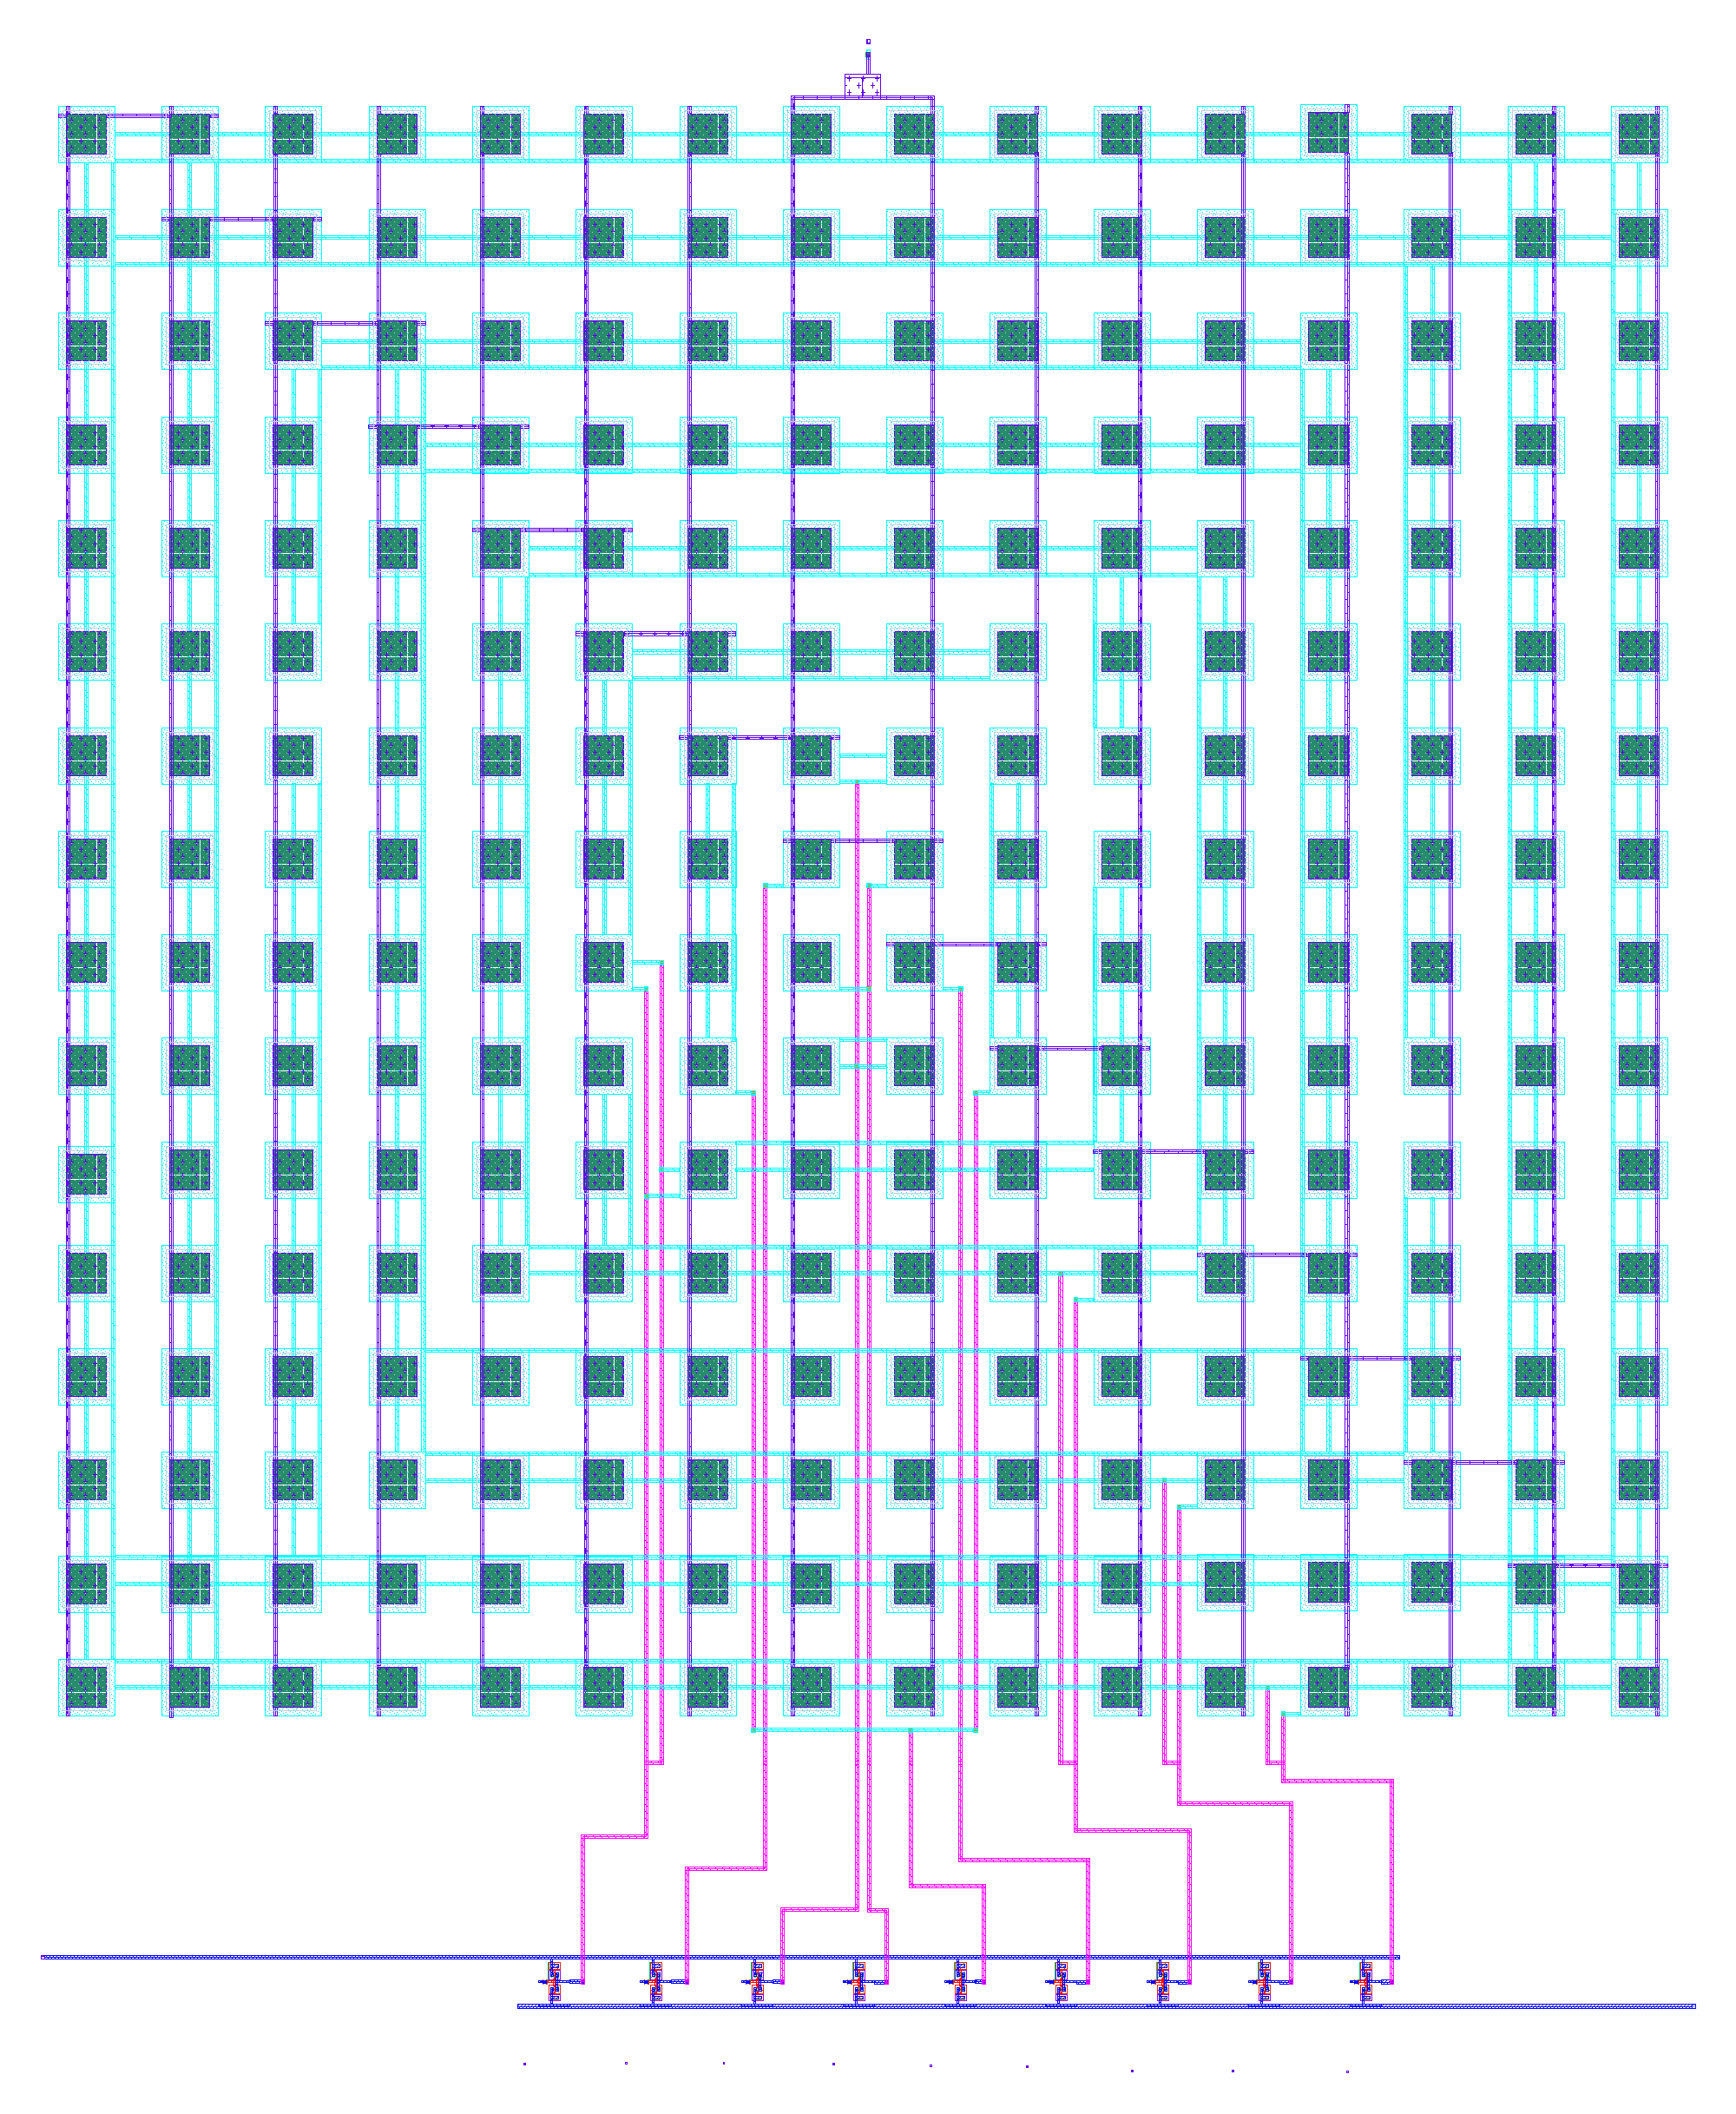
\includegraphics[width=2.4cm]{fig/cdac_8b.png}};
  \node[font=\scriptsize,anchor=north,align=center] at (11.1,3.55) {\textbf{CDAC}: 8-bit array + drivers\\ 140.6 $\times$ 172.7\,$\mu$m};
  \node[anchor=south west,inner sep=0] at (12.9,5.0) {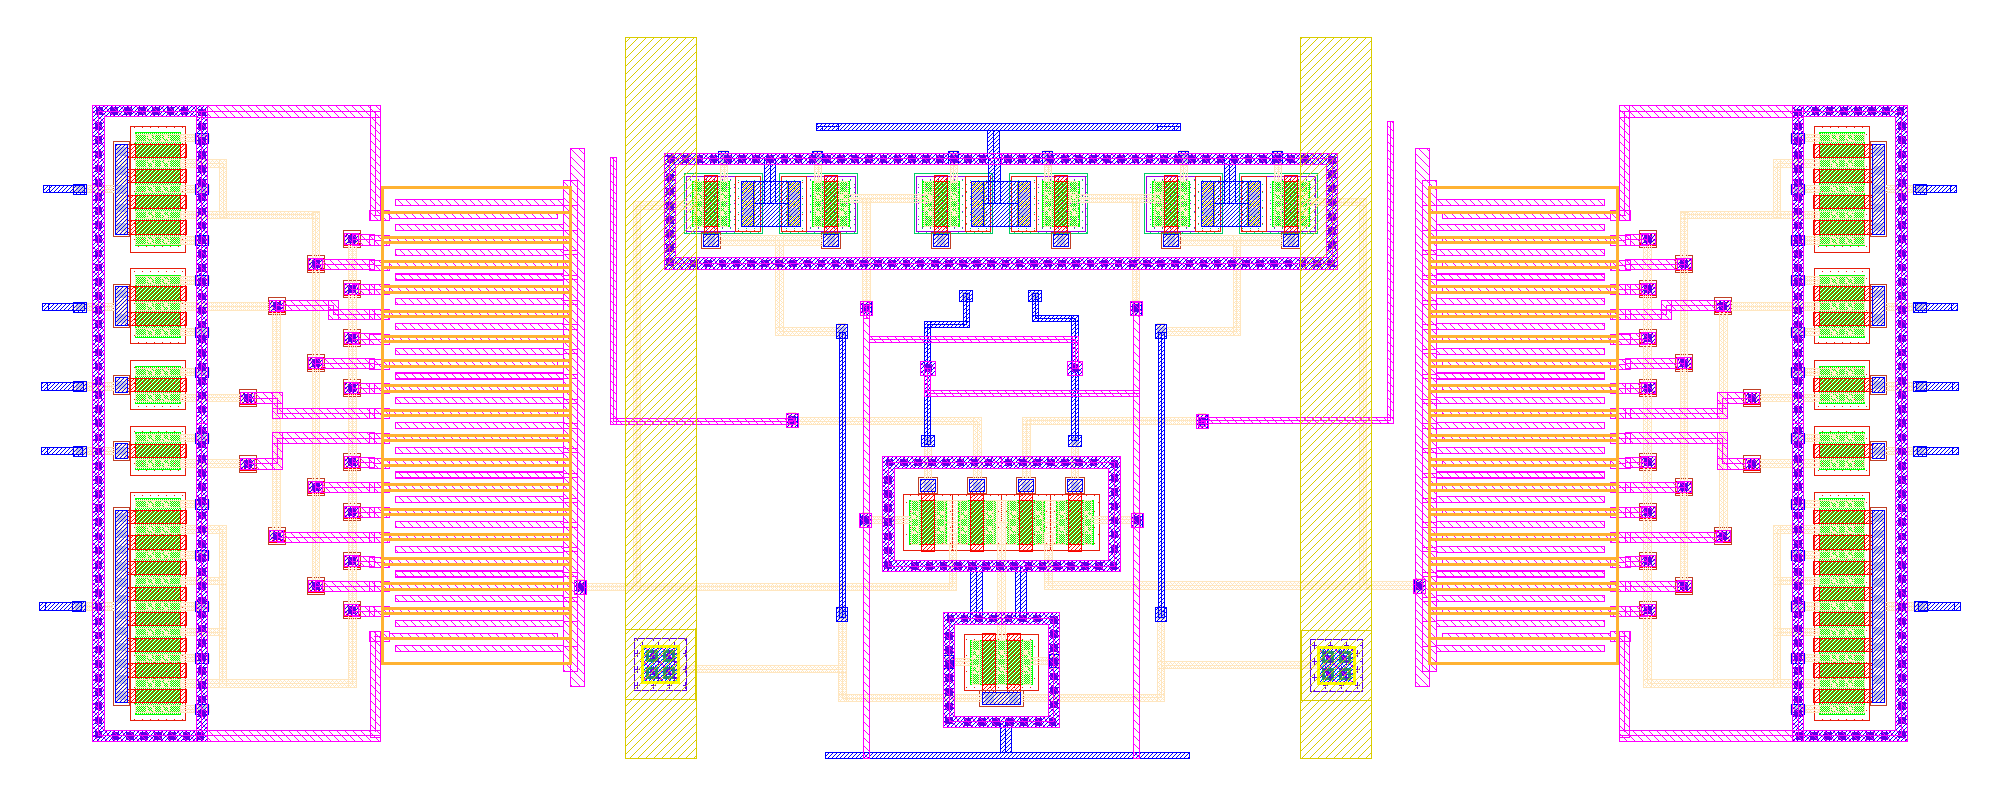
\includegraphics[width=4.4cm]{fig/comparator.png}};
  \node[font=\scriptsize,anchor=north,align=center] at (15.1,4.95) {\textbf{comparator} --- 43.4 $\times$ 16.3\,$\mu$m};
  \node[anchor=south west,inner sep=0] at (12.9,2.75) {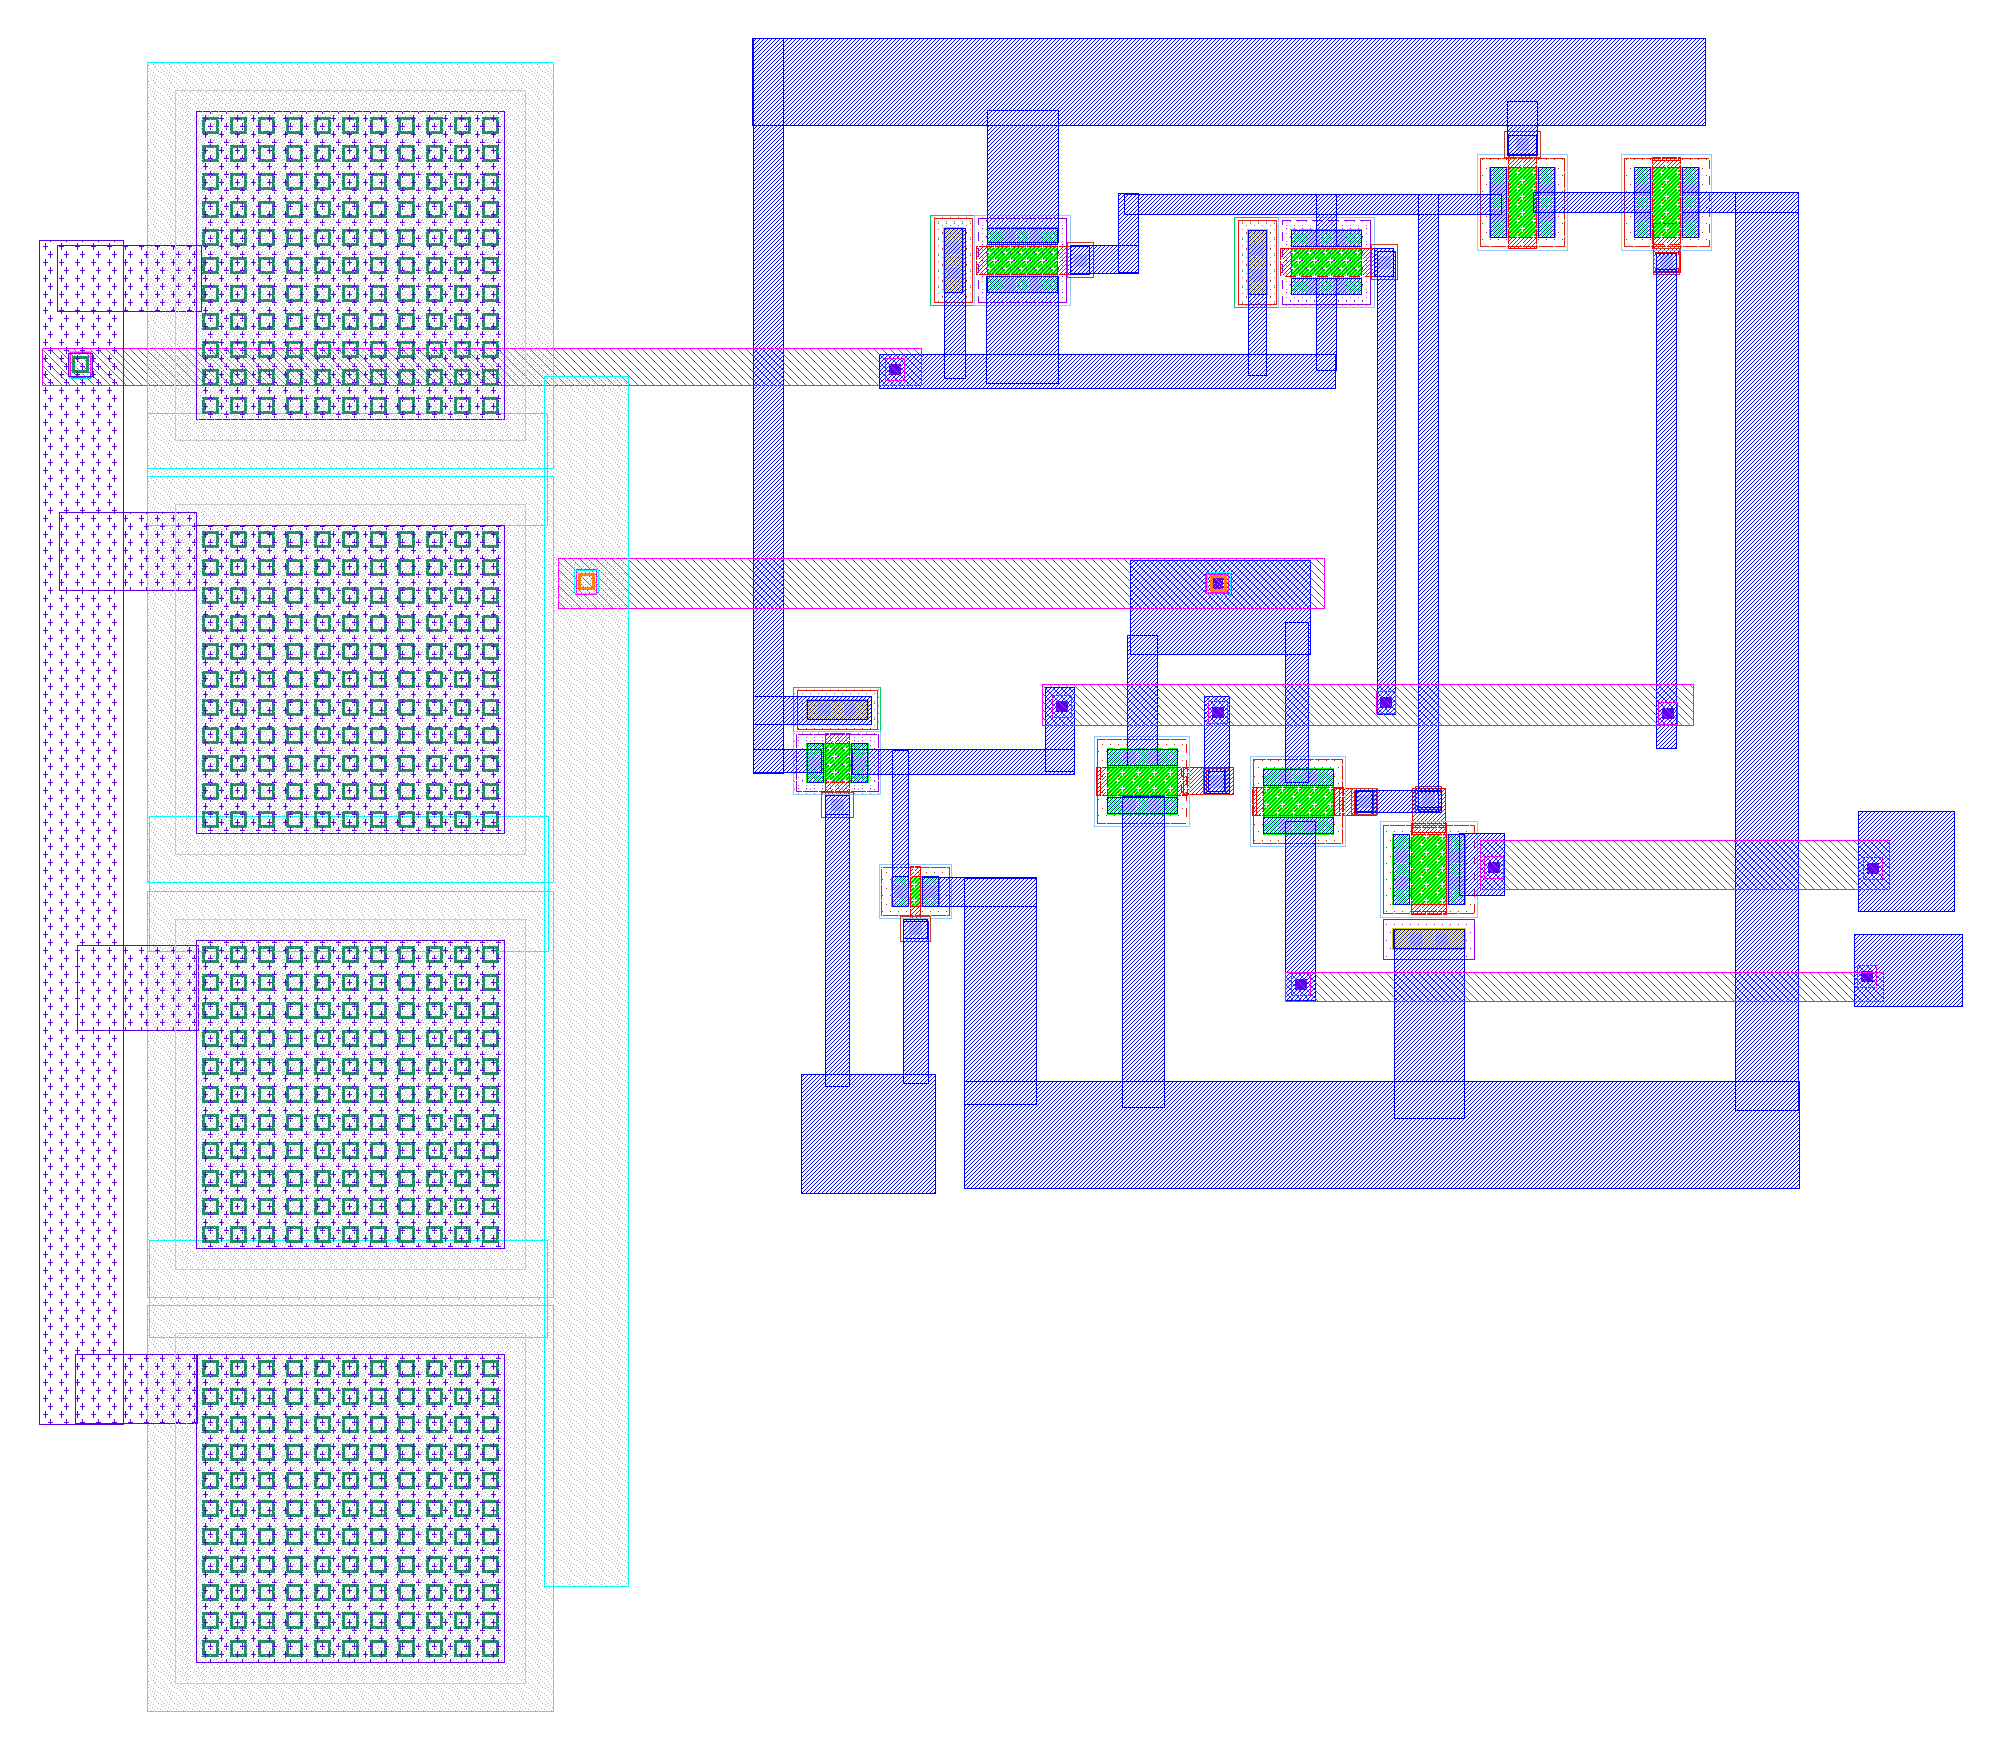
\includegraphics[width=1.9cm]{fig/bootstrap_sw.png}};
  \node[font=\scriptsize,anchor=north,align=center] at (13.85,2.7) {\textbf{bootstrap switch}\\ 27.5 $\times$ 23.9\,$\mu$m};
  \node[anchor=south west,inner sep=0] at (15.7,2.9) {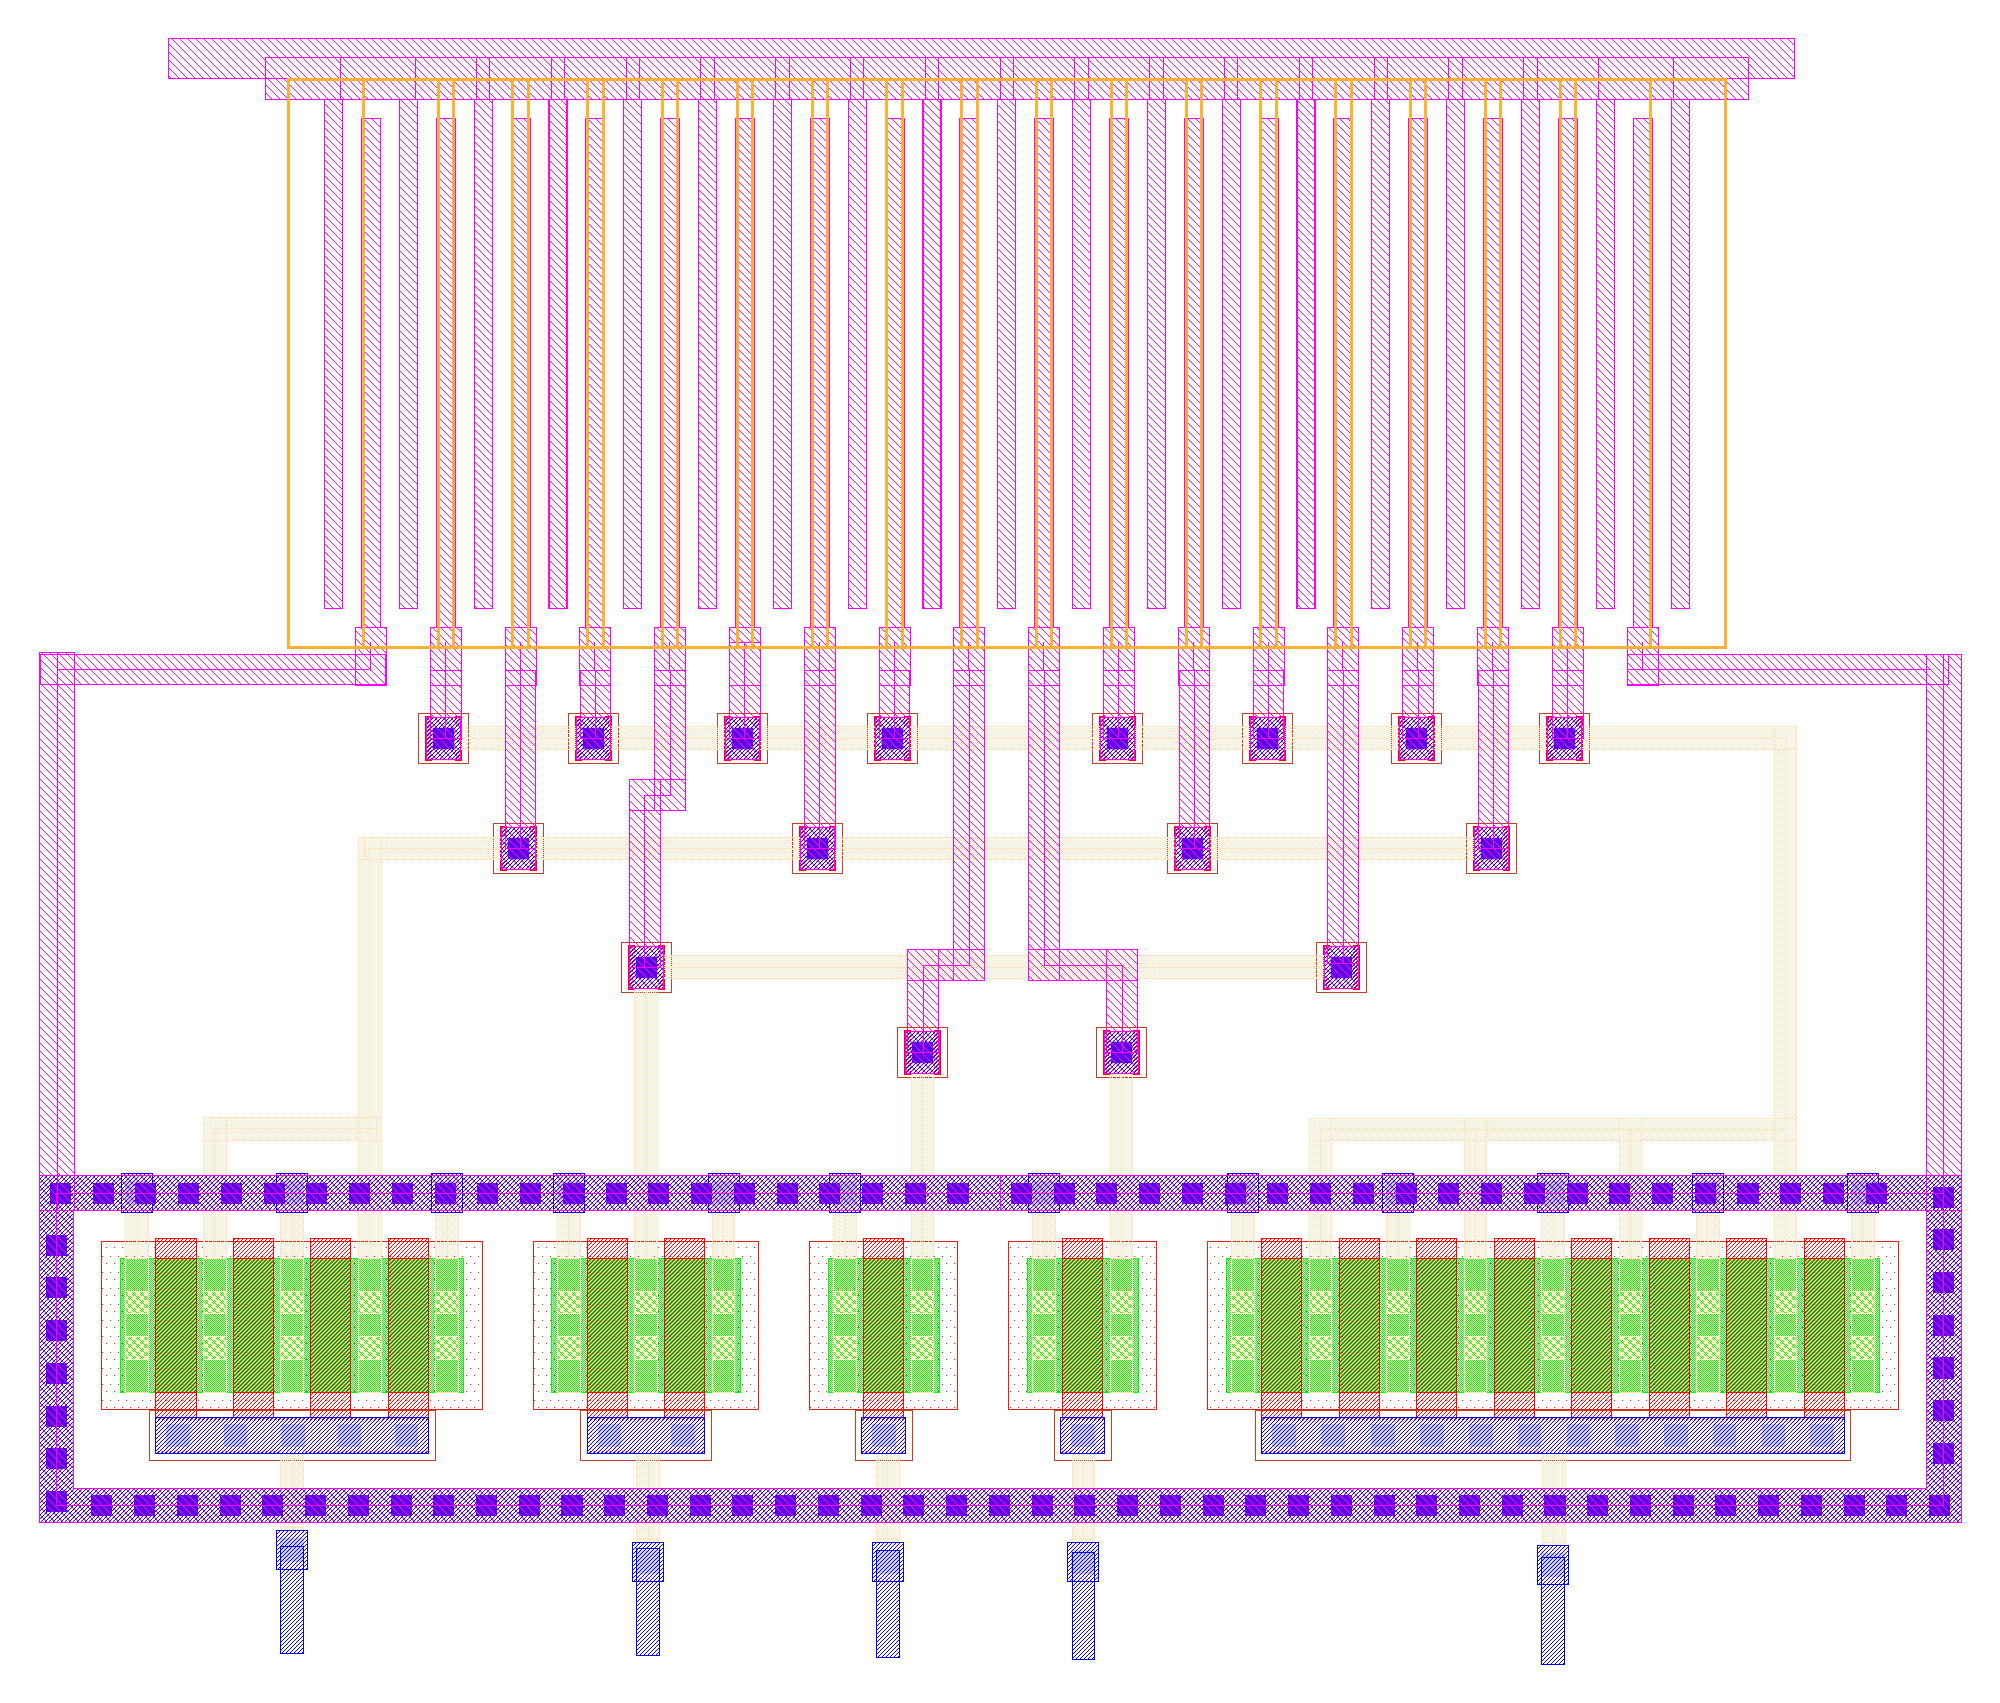
\includegraphics[width=1.6cm]{fig/trim.png}};
  \node[font=\scriptsize,anchor=north,align=center] at (16.5,2.7) {\textbf{trim array}\\ 14.4 $\times$ 12.2\,$\mu$m};
  \node[font=\scriptsize,anchor=north west,align=left,text width=7.8cm] at (9.9,1.9) {The complete analog front end occupies $\approx$0.03\,mm$^2$ --- under 0.3\,\% of the 10.3\,mm$^2$ core. Cells rendered from the sky130 GDS (comparator, trim: Erick; CDAC: Hee; switch: Jaime).};
\end{tikzpicture}}\\[1pt]
\parbox{\textwidth}{\footnotesize\textbf{Fig.~2.} Left: the routed SoC as of 21 Sep, post-route with filler, pre-signoff (filler cells and row rails hidden for clarity): 3.44\,$\times$\,4.04\,mm die, SKY130 pad ring, four 8\,kB SRAMs, Cortex-M0 (red), fabric logic. Right: four analog cells, enlarged.}
\end{center}

\section{Milestone 1 Status}
\small
\begin{tabularx}{\textwidth}{@{}l l l l X@{}}
\toprule
\textbf{Cell} & \textbf{Owner} & \textbf{DRC} & \textbf{LVS} & \textbf{Open item} \\
\midrule
inverter & Hee & \ok & \okm & --- \\
cap array (carray\_8b) & Hee & \ok & \mm & schematic/layout unit-cap count to reconcile (127 vs 128) \\
CDAC (cdac\_8b) & Hee & \ok & \nr & --- \\
bootstrap switch & Jaime & \ok & \mm & recharge under rapid triggering to characterise \\
comparator & Erick & \ok & \mm & layout pin labels \\
trim array & Erick & \ok & \nr & ideal caps to be replaced by SKY130 MIM \\
\bottomrule
\end{tabularx}
6 of 6 cells DRC-clean (exc. density rules, to be resolved by chip fill in integration).  1 of 6 LVS-matched. Firmware regression: 6/6.
\normalsize

\section{Verification Plan}
\small
\begin{tabularx}{\textwidth}{@{}l X X X@{}}
\toprule
\textbf{Level} & \textbf{Physical} & \textbf{Electrical} & \textbf{System} \\
\midrule
ADC macro & DRC/LVS clean, parasitics extracted & ADC FOM simulated: INL/DNL, ENOB across corners & Extracted netlist passes the AMS testbench regression tests\\
Chip & Full-chip DRC, LVS, ERC, antenna, fill & Static timing at 33\,MHz post-route (done); review with mentors & All firmware tests pass in AMS + gate level simulation \\
\bottomrule
\end{tabularx}
\normalsize

\section{Risks and Mitigation Plan}
\small
\begin{tabularx}{\textwidth}{@{}l X@{}}
\toprule
\textbf{Risk} & \textbf{Mitigation} \\
\midrule
ADC misses spec & Digital SoC is already timing-closed and firmware-verified: silicon returns as a working Cortex-M0 MCU regardless and the ADC is characterisable via the firmware. \\
ADC switch recharge limits rate & Increase the minimum conversion interval in firmware. \\
Comparator offset exceeds trim & Cap sizing reviewed by Kushal Das in M1, before the layout is frozen. \\
Schedule slip & Two weeks of buffer time before 7~Dec. \\
\bottomrule
\end{tabularx}
\normalsize

\section{Physical Test Plan}
\small ChipFoundry's chipIgnite delivers 100 QFN parts, an evaluation board and 10 parts on M.2 cards five months after tapeout (\textasciitilde May 2027). Bring-up procedure: (1) boot the Cortex-M0 over SWD with the regression firmware images; (2) characterise the ADC from a signal generator through the same firmware sensing tests and measure key FOM (INL/DNL from a slow ramp, ENOB from an FFT of captured codes); (3) report to S3B and the SoCLabs contest.

\section{Resourcing}
\vspace{-5pt}\small
\begin{minipage}[t]{0.5\textwidth}
\vspace{0pt}
\begin{tabularx}{\textwidth}{@{}l X r@{}}
\toprule
\textbf{Who} & \textbf{Role} & \textbf{h/wk} \\
\midrule
Lewis Watts & Lead; & 5 \\
Daniel Geng & Synthesis and place-and-route & 10 \\
Hee Chan Kim & Capacitor array, CDAC, analog library & 10 \\
Erick Gomez & Comparator, offset-trim arrays & 12 \\
Jaime Pryor & Bootstrap sampling switch & 8 \\
Benjamin Schwarz & Digital verification & 5 \\
\midrule
\multicolumn{3}{@{}l@{}}{\footnotesize\textbf{Supervisor:} Prof.\ Philip Leong. \textbf{External reviewers:} see Sec.~1.} \\
\bottomrule
\end{tabularx}
\end{minipage}\hfill
\begin{minipage}[t]{0.46\textwidth}
\vspace{0pt}
\textbf{Summary.} Key infrastructure risks including synthesis, place-and-route, AMS co-simulation and extraction all working. Remaining tasks include analog block LVS, macro layout and integration. Our work will continue to be reviewed periodically by three external engineers.
\end{minipage}
\normalsize

\end{document}
